\subsubsection{Enzyme Design}
\index{Jeltsch, Albert}

\paragraph{Research Team}
%
Albert Jeltsch (Professor),
Sandra Becker (Technician),
Sanjay Chahar (PhD Student),
Arunkumar Dhayalan (PhD Student),
Renata Jurkowska (PhD Student),
Tomek Jurkowski (PhD Student),
Heike Laser (Postdoc),
Kirsten Liebert (Postdoc),
Sergei Ragozin (Postdoc),
Philipp Rathert (PhD Student),
Christian Rohde (PhD Student),
Martina Schlickenrieder (PhD Student),
Maike Schwerdtfeger (Lab Technician),
Yinying Zhang (PhD Student)\\

%Albert Jeltsch, Prof. Dr., Prof. of Biochemistry,
%Sandra Becker, Technician,
%Sanjay Chahar, M.Sc., PhD student,
%Arunkumar Dhayalan, M.Sc., PhD student,
%Renata Jurkowska, M.Sc., PhD student,
%Tomek Jurkowski, M.Sc., PhD student,
%Heike Laser, Dr., PostDoc,
%Kirsten Liebert, Dr., PostDoc,
%Sergei Ragozin, Dr., PostDoc,
%Philipp Rathert, Dipl. Biol., PhD student,
%Christian Rohde, Dipl. Biol., PhD student,
%Martina Schlickenrieder, Dipl. Biol., PhD student,
%Maike Schwerdtfeger, Technician,
%Yinying Zhang, M.Sc., PhD student\\

The research of my group in the field of Biotechnology and protein design focuses on the following projects: i) We aim to design DNA methyltransferases that can be employed for targeted methylation of the human genome. This approach could lead to a novel approach to shutdown the expression of genes in vivo which could have a wide range of applications in the future including treatment of cancer and viral infections. ii) We apply methods of directed and evolutionary protein design to generate DNA methyltransferase with improved properties for various applications.  iii) Based on our expertise in protein design and directed evolution approaches we develop general method for biotechnological applications.

\paragraph{Highlights}
%
Gene silencing by targeted DNA methylation has potential applications in basic research and therapy. To establish targeted methylation in human cell lines, the catalytic domains of mouse Dnmt3a and Dnmt3b DNA methyltransferases (MTase) were fused to different DNA binding domains of GAL4 and an engineered zinc finger domain. In collaboration with M. Papworth (Cambridge, UK) and F. Li (Shanxi, China) we demonstrated that
\begin{enumerate}
\item { Dense DNA methylation can be targeted to specific regions in gene promoters using chimeric methyltransferases.}
\item { Site-specific methylation leads to repression of genes controlled by various cellular or viral promoters.}
\item { Mutations affecting any of the DNA binding domains, MTase or target DNA sequences reduce targeted methylation and gene silencing.}
\item { Targeted DNA methylation is effective in repressing HSV-1 infection in cell culture with the viral titer reduced by at least 18-fold in the presence of an MTase fused to an engineered zinc finger DBD, which binds a single site in the promoter of HSV-1 gene IE175k.}
\end{enumerate}
Our results demonstrate that it is possible to direct DNA methyltransferase activity to predetermined sites in DNA, achieve targeted gene silencing in mammalian cell lines and interfere with HSV-1 propagation.

\begin{figure}[ht]
  \begin{center}
   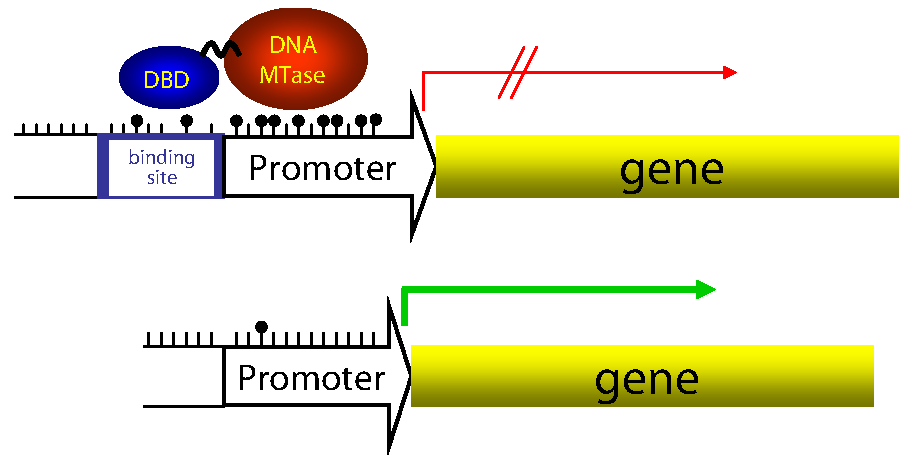
\includegraphics[width=\hsize]{Jeltsch/Fig_Jeltsch2_2006.pdf}
    \mycaption{Schematic drawing of the specific methlytion of DNA by DNA binding domain-DNA MTase fusion proteins.}\label{Fig_Jeltsch2_2006.pdf}
   \end{center}
\end{figure}


Protein/protein interaction is an essential process in cellular physiology. In addition, protein/protein interaction sites are potentially important drug targets, because manipulation of protein/protein interaction will allow for a specific interfer-ence will cellular metabolism and regulation. Therefore, mapping of the interfaces of protein complexes is an important task. We have developed a general system that allows us to deine the residues involved in protein/protein interaction for any pair of proteins. In the first step a yeast-two hybrid construct is prepared for the pair of proteins to be analyzed. Such systems are already established for many protein pairs due to various high-throughput projects aiming to identify protein/protein interaction. In the next step, one of the two partners is subjected to high-level randomization and the library selected for clones that still do interact. These clones are sequenced. Since the amino acid exchanges observed in such clones did not interfere with protein/protein interaction, they will provide a negative footprint of the interaction region, where mutations are excluded. This method may be useful for large scale high throughput mapping of protein/protein interaction sites.\newline \newline Albert Jeltsch is also involved in ``Biochemistry - Methyltransferases''.


\myparagraph{Collaborations}
%
Bremen Area Collaborations:
\begin{enumerate}
%
\item {\sl International University Bremen} \\ Prof. K. Brix \\ Confocal cell imaging
 \\ Prof. G. Mushkelishvili \\ AFM of DNA methyltransferases
 \\ Prof. W. Nau \\ Investigation of Peptide Dynamics
\\ Prof. S. Springer \\ Rapid Kinetics
\\ Dr. H. Stamerjohanns \\ Data analysis and web programming
 \\ Prof. M. Ullrich \\ Mass spectrometry
 \\ Dr. C. Voelcker-Rehage \\ Genkotyping participants of the JC aging study
 \\ Prof. M. Winterhalter \\ Dynamic light scattering
 \\ Prof. M. Zacharias \\ Simulation of enzyme dynamics
\end{enumerate}
National \& International Collaborations:
\begin{enumerate}
\item {\sl University of Texas, Department of Carcinogenesis, Smithville, Texas, USA} \\ Prof. M.T. Bedford \\ Peptide interaction of DNA methyltransferases
\item {\sl Emory University Atlanta, Department of Medicine, GA, USA} \\ Prof. X. Cheng \\ X-ray crystallography and inhibitor design of DNA methyltransferases
\item {\sl Universit�t Halle} \\ Prof. R. Dammann \\ Expression of Dnmt1 in cells
\item {\sl University of Edinburgh, Edinburgh, UK} \\ Prof. D.T.F. Dryden \\ Time resolved fluorescence spectroscopy with DNA methyltransferases
\item {\sl Laboratory of Cancer Epigenetics, Faculty of Medicine, Free University of Brussels, Brussels, Belgium} \\ Prof. F. Fuks \\Phosphorylation of DNA methyltransferases
\item {\sl DKFZ, Heidelberg} \\ Prof. I. Grummt \\ Regulation of DNA methyltransferases in cells
\item {\sl Hungarian Academy of Science, Szeged, HU} \\ Prof.  A. Kiss \\ Expression and Design of the M.SssI DNA methyltransferase
\item {\sl Department of Biochemistry and Molecular Biology, University of Shaanxi, China} \\ Dr. F. Li \\Targeted methylation of DNA in cells
\item {\sl DKFZ, Heidelberg} \\ Dr. F. Lyko \\ Expression and characterisation of Dnmt2
\item {\sl University of Groningen, Groningen, The Netherlands} \\ Dr. P. McLaughlin\\ Targeted methylation of DNA in cells
\item {\sl National Cancer Institute, Frederick, MD, USA} \\ Prof. K. Muegge \\ Regulation of Dnmt3a in cells
\item {\sl Institut f�r Genetik, Universit�t Kassel} \\Prof. W. Nellen \\ Expression and characterisation of Dnmt2
\item {\sl The Wellcome Trust Biocentre, University of Dundee, Dundee, UK} \\ Prof. T. Owen-Hughes \\ Preparation of nucleosomal DNA
\item {\sl MRC, Cambridge, UK} \\ Dr. M. Papworth\\ Targeted methylation of DNA in cells
\item {\sl Leibnitz Institute for Age Research, Jena} \\ Dr. M. Platzer \\ High troughput DNA Sequencing
\item {\sl Justus-Liebig Universit�t Giessen} \\ Prof. A. Pingoud \\ Targeted DNA cleavage
\item {\sl MPI f�r Molekulare  Genetik, Berlin }\\ Dr. R. Reinhardt \\ High troughput DNA sequencing
\item {\sl CNRS/University of Rennes 1 Joint Unit, Rennes, France} \\ Dr. G. Salbert \\ Enzymology of Dnmt3a
\item {\sl MHH, Hannover \\ Prof. C. Urbanke} \\ Analytical Ultracentrifugation
\item {\sl Universit�t Saarbr�cken} \\ Prof. J. Walter \\Human Methylome analysis
\item {\sl Chinese Academy of Sciences, Shanghai, China} \\ Prof. G. Xu \\ Biologcial role of Dnmt3a
\end{enumerate}

\paragraph{Organization}
%
\begin{enumerate}
\item {Member of the editorial board of BMC Biochemsitry}
\end{enumerate}

\newpage
\paragraph{Grants}
\begin{enumerate}
\item
Funded by BMBF, \emph{Biofuture. Development of programmable DNA methyltransferases for
  biotechnological applications }, (August 2003 - Dezember 2007)

\item
Funded by BMBF, \emph{BioChancePlus. Amplification of DNA with preservation of the
  methylation state }, (May 2004 - April 2007)

\item
Funded by BMBF, \emph{SMP Epigenetics. Analysis of the DNA methylation pattern of genes on
  Chromosome 21 }, (May 2005 - April 2007)

\item
Funded by NIH (USA), \emph{Histone Lysine Methylation: structures and functions},
GM068680-01A2, (October 2006 - September 2011)

\item
Funded by DFG, \emph{Directed evolution of DNA methyltransferases}, priority program
SPP1070, JE252/5-1 and 5-2, (September 2004 - May 2007 (JE252/5-1), December 2006 -
December 2008 (JE252/5-2))

\item
Funded by DFG, \emph{Biochemistry and biological function of mammalian Dnmt1 and Dnmt2},
priority program SPP1129, JE252/4-2 and 4-3, (December 2005 - November 2007 (JE252/4-2),
October 2006 - December 2008 (JE252/4-3))

\item
Funded by DFG, \emph{Enzymology, structure and DNA recognition of the E. coli dam DNA
  methyltransferase}, JE252/2-6, (October 2005 - December 2008)

\end{enumerate}

\paragraph{Other Support Grants}
\begin{enumerate}
\item {JE252/2-5 (DFG) ``Enzymology, structure and DNA recognition of the E. coli dam DNA methyltransferase'' at University of Gie\ss en}
\item {HBFG 066/7-1 (DFG) ``Purchase of a MALDI TOF mass spectrometer''}
\end{enumerate}

\paragraph{Patents}
\begin{enumerate}
\item {Patent application: Pingoud, Jeltsch, Eisenschmidt: Hochspezifisch mit DNA interagierende Enzym-Konjugate. EPA 2005/009028 (pending)}
\item {Cheng, Horton, Yang, Calman, Zhang, Jeltsch, Hattmann ``Small Molecule Inhibitors of Bacterial Dam DNA Methyltransferases'', PCT Patent Application No. PCT/US 05/44277, 2006 (pending)}
\end{enumerate}


\paragraph{Awards, Prices}
\begin{enumerate}
\item {Elected as vice-president of the DNA Methylation Society (New Orleans, LO)}
\end{enumerate}


\nocite{Jeltsch1,Jeltsch2,Jeltsch3,Jeltsch4,Jeltsch5,Jeltsch6,Jeltsch7,Jeltsch8,Jeltsch9,Jeltsch10}
